\chapter{团队建立}\label{sec:report-team}

我们是天津大学软件学院 2024 级的四名本科生，共同完成了轻量级外卖服务平台的需求分析、设计、开发、测试和部署。小组按模块分工，联调时沿同一笔外送订单核对顾客、商家、骑手和管理员的操作衔接。项目代码托管在 GitHub 的 \texttt{lightweight-takeout-platform} 仓库。

\section{团队成员}

\paragraph{组长李承文（学号 3024232129）}
李承文担任项目经理和 Scrum Master，安排迭代、组织 PR 评审并负责部署。他维护 \code{elm_bk} 的认证、交易、资产、配送和管理端服务。后端使用 Java 17 和 Spring Boot 3.4.6，由 Spring Security 和 JWT 校验角色权限，通过 MyBatis 执行库存扣减和配送任务的条件更新。他还维护演示脚本和 \code{docker-compose.demo.yml}。

\paragraph{组员范文丽（学号 3024244438）}
范文丽负责顾客、商家和管理员的界面，代码位于 \mbox{\code{elmclient/src/views/}}。她维护 \mbox{\code{AiChat.vue}}、主题和数据看板。页面用 Vue 3 Composition API 管理状态，通过 Vue Router 限定各角色的页面入口，由 Axios 统一处理请求和异常。界面支持四套 CSS 变量主题、转场和窄屏适配，数据看板使用 ECharts/SVG 并支持 Excel/PDF 导出。

\paragraph{组员赵紫怡（学号 3024244137）}
赵紫怡兼任产品负责人，负责需求分析和数据库设计。她主编 \code{docs/SRS.pdf} 及飞书需求文档，用 UML 和 draw.io 描述各端用例，维护 MySQL 8 基线 \code{elm_bk/db/schema/elm_v2.sql} 与 \code{001}--\code{006} 迁移脚本。AI 点餐后端也由她负责。她维护 \mbox{\code{AiChatController}}、\mbox{\code{AssistantController}} 和多模态客户端，接入 DeepSeek 与 DashScope。

\paragraph{组员仲禹潼（学号 3024244140）}
仲禹潼负责质量保障和交叉验收，按等价类与边界值设计用例，通过 JUnit 5、MockMvc 和 Node 测试运行器复测，并在 WPS 台账登记缺陷。他负责地图功能，连接 \code{MapController}、\code{MapLocationPicker} 选址弹窗与 \code{RiderDashboard.vue} 的导航入口。选址使用 POI 检索和逆地理编码，骑手侧按 GCJ-02 坐标估算距离。

飞书保存需求与站会结论，涉及多个模块的决定在腾讯会议上讨论。GitHub 保留代码与评审意见，WPS 台账记录缺陷的复现步骤和复测结果。图~\ref{fig:team-topology} 列出了各项记录的维护人和成员之间的交接关系。

\begin{figure}[!htbp]
  \centering
  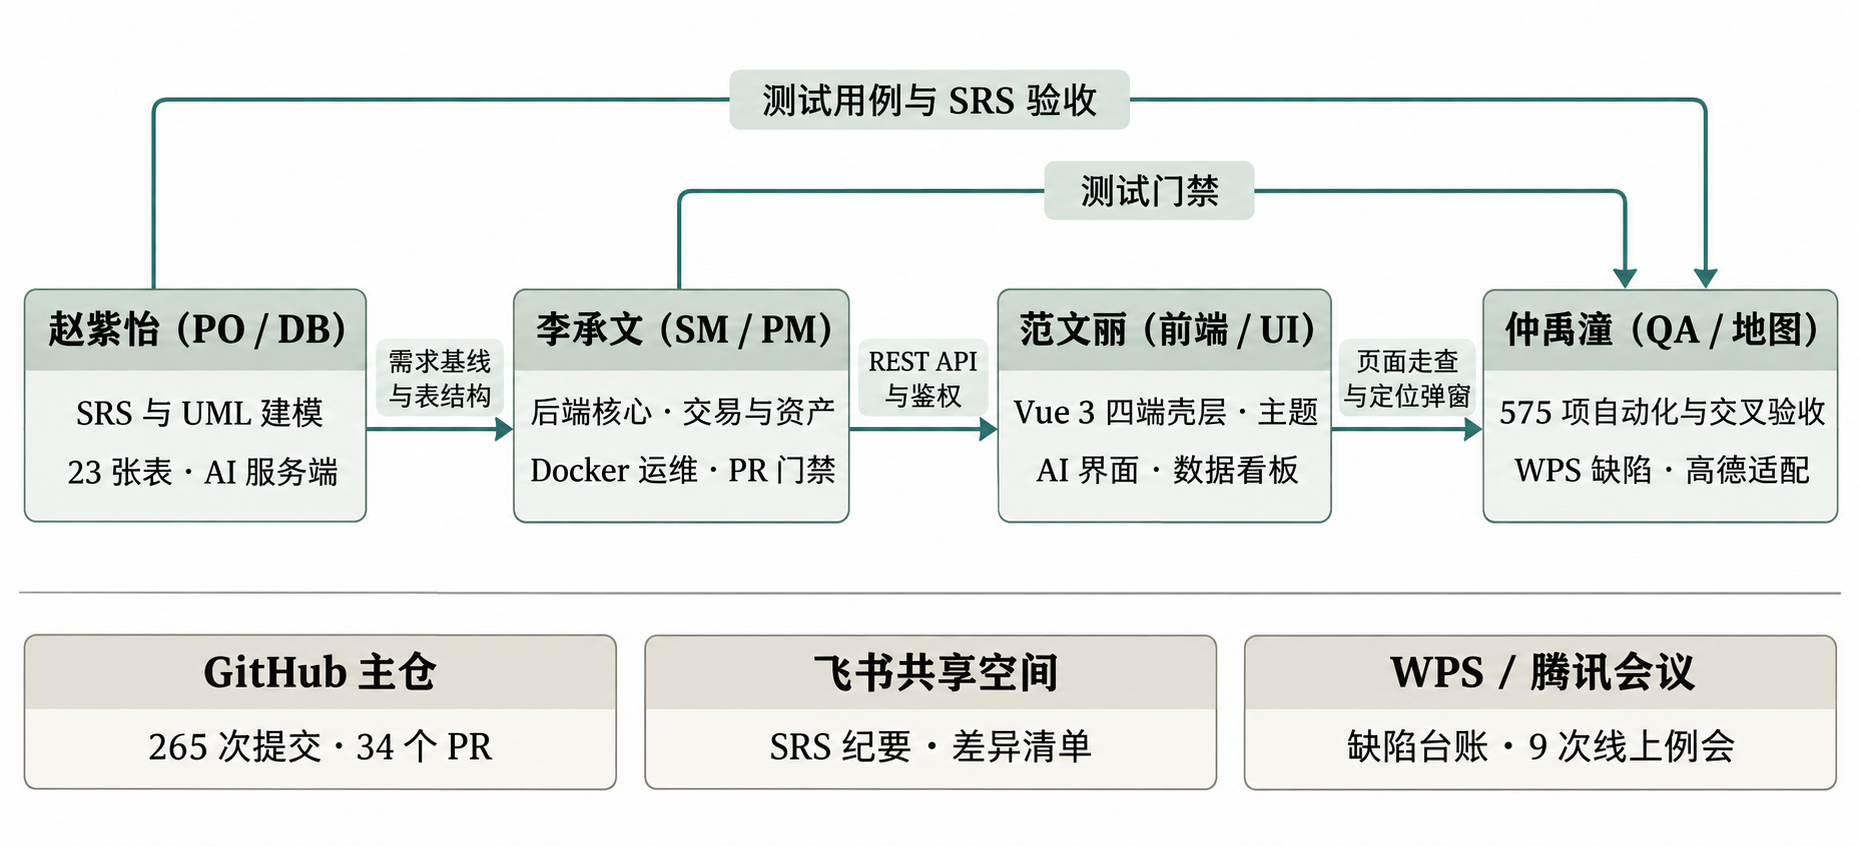
\includegraphics[width=.98\linewidth]{figures/report/process/team-handoff.png}
  \caption{小组成员角色分工与工程协作基础设施拓扑图}\label{fig:team-topology}
\end{figure}

店铺营业状态需要商家与顾客两端协作。需求约定\textbf{休息中的店铺保留菜单展示，暂停接收新订单}。商家提交后，后端保存状态并在加购和建单时检查，顾客端显示“休息中”。验收时用两个账号操作同一家店，分别核对商家保存的营业状态和顾客端的下单限制。

\section{团队角色与任务分配}

\subsection{需求、迭代与交付}

赵紫怡按 P0、P1 和 P2 将用例纳入 Product Backlog，在 SRS 中写明各角色的操作、异常处理和验收条件。团队评审系统上下文图、四端用例图、领域类图和状态机图时，把发现的状态命名差异记入飞书，在 SRS 2.0 中统一。迭代评审时，她再用需求里的用例检查已实现功能。

李承文将任务分到三个 Sprint，设置里程碑，组织站会、评审和回顾。前后端的字段或状态含义出现分歧时，他召集成员确认接口约定，再安排调整和联调。他负责主干保护、PR 评审和合并冲突处理，维护 \code{scripts/check-repository.mjs} 与容器演示环境，并在交付前核对风险台账、测试记录和部署材料。

\subsection{开发与联调}

四类角色各有页面入口，共用路由、主题及请求处理。范文丽负责页面组织和公共壳层，主要维护 \code{Index.vue}、\code{BusinessInfo.vue}、\code{Cart.vue}、\code{OrderList.vue}、\code{AiChat.vue}、\code{Preferences.vue} 以及商家和管理员看板。仲禹潼协作完成 \code{MapLocationPicker}、地址与地图联动，以及骑手工作台 \code{RiderDashboard.vue} 的导航入口。两人共同核对地址字段、\mbox{选址异常提示和窄屏布局}。

后端按 Controller、Service、Mapper 分层。李承文负责登录、角色切换和履约状态更新，也维护订单提交、计价、结算和资产服务，分别对应 \mbox{\code{OrderSubmissionService}}、\mbox{\code{OrderPricingService}}、\mbox{\code{OrderSettlementService}} 和 \mbox{\code{AssetService}}。订单提交、取消回滚、资产扣减和骑手接单都需要核对权限、幂等和事务边界。

赵紫怡维护对话和结构化助手服务，分别由 \mbox{\code{AiChatServiceImpl}} 和 \mbox{\code{StructuredAssistantServiceImpl}} 实现。她还维护 \mbox{\code{AiRecommendationServiceImpl}}，对接模型适配器和商家菜单查询。外部服务异常时，系统切回本地处理。

赵紫怡设计了 23 张核心业务表及主外键、查询索引，李承文协作处理迁移和并发更新。两人把成交时的商品、地址快照与商家的可变配置分开存储，维护订单、配送、资产流水、评价、通知和 AI 对话等表，并为账号唯一性、默认地址、菜品快照、备注和地图坐标编写版本化迁移。

\subsection{质量保障}

每轮功能完成后，仲禹潼先用四类账号检查页面和接口，再测试库存边界、密码、越权和定位异常。WPS 台账逐条记录缺陷所在模块、复现顺序、截图与复测结果。容易复发的问题写入自动化测试，开发者提交前运行，合并时由同伴复核。

回归中，后端 53 个 JUnit/MockMvc 测试类有 340 项通过，前端 28 个 Node 测试文件有 235 项通过。仲禹潼还组织人工走查与跨组交叉验收。表~\ref{tab:team-matrix} 列出成员分工和联调重点，附录表~\ref{tab:code-ownership} 记录主要代码与文档的归属。

\begin{longtable}{L{.09\linewidth}L{.155\linewidth}L{.24\linewidth}L{.455\linewidth}}
\caption{小组成员角色、扩展模块与协作接口矩阵}\label{tab:team-matrix}\\
\toprule
\textbf{成员} & \textbf{基础主责方向} & \textbf{Scrum/专项模块} & \textbf{协作接口与联调关注点} \\
\midrule
\endfirsthead
\multicolumn{4}{c}{{\tablename\ \thetable{} 续表}}\\
\toprule
\textbf{成员} & \textbf{基础主责方向} & \textbf{Scrum/专项模块} & \textbf{协作接口与联调关注点} \\
\midrule
\endhead
\bottomrule
\endfoot
范文丽 & 前端开发 & UI 主题、数据看板 & 对齐后端响应字段与页面状态，实现四端界面、主题切换与经营/平台看板可视化。 \\
李承文 & 后端开发 & 组长/SM、红包积分 & 统筹进度和 PR 合并，衔接订单定价、支付、优惠券、积分与钱包流水回退规则。 \\
赵紫怡 & 数据库设计 & PO/SRS、AI 点餐 & 主编 SRS 与数据模型，对接真实菜单、订单权限校验和多模态 AI 服务。 \\
仲禹潼 & 测试工程 & QA 负责人、高德地图 & 组织回归测试与交叉验收，验证地图选址、距离估算、骑手导航与降级场景。 \\
\end{longtable}

\section{培训大纲}

四人各有熟悉的方向，联调缺陷常同时涉及页面、服务和数据。培训先练习搭建环境、建分支和登记缺陷，要求每人在自己的电脑上走完一笔订单，再\mbox{按分工开展专题练习}。

\subsection{培训目标}

\begin{reportpoints}
\item 用 Scrum 组织迭代，结合课程讨论的需求管理、项目策划、验证和确认做法，对应 REQM、PP 和 VER/VAL。站会记录待处理事项，合入前审查代码，修复后按原步骤复测。
\item 每人能独立运行 Vue 3 前端、调试 Spring Boot 后端、初始化 MySQL 容器并执行测试。协作时统一使用 GitHub 特性分支和 PR，飞书与腾讯会议保存结论，WPS 台账登记缺陷，Playwright 和 Chrome 用于走查页面。
\item 选用服务端计价、JWT 身份读取、订单快照和外部服务超时练习 TDD。先用失败用例复现问题，再修改实现，最后用同一组用例保障整理后的代码行为。
\end{reportpoints}

\subsection{培训对象与分层重点}

全员先走读点餐至履约的四端流程，练习启动环境、认领任务、提交改动和归档。范文丽与仲禹潼随后练习路由守卫、CSS 变量主题、地图弹窗、响应式适配和前端单测。李承文与赵紫怡走读 MyBatis 映射，练习条件更新、事务回滚、\code{BigDecimal} 算价、历史快照和外部接口适配。仲禹潼与李承文把关键用例整理为可重复运行的回归测试，并练习 Nginx 代理与部署排查。分层安排见表~\ref{tab:training-roles}。

\subsection{培训内容与实施计划}

启动会上，李承文和赵紫怡通过腾讯会议讲解课程交付要求，演示如何从用户故事找到对应的图、接口和测试，并统一站会日志与缺陷登记字段。首轮开发前，范文丽示范 Vue 3 目录、Axios 拦截器和组件拆分，李承文讲解后端分层，赵紫怡带领组员阅读 \code{elm_v2.sql} 和迁移约定。李承文演示分支、PR 和 Docker Compose，仲禹潼检查组员能否在各自环境运行 \code{./mvnw test} 与 \code{npm test}。

交易规则训练以购物车多选结算、防超卖库存扣减和积分抵扣为例。赵紫怡和仲禹潼分别讲解 DeepSeek/DashScope 降级与高德坐标转换。测试训练将库存溢出、跨用户数据隔离整理成可重复执行的用例。联调中遇到异步竞态、返回循环和窄屏溢出时，组员开短会并一起查代码。早期演练的操作和检查条件见表~\ref{tab:training-labs}。

\begin{longtable}{L{.20\linewidth}L{.42\linewidth}L{.34\linewidth}}
\caption{团队工程实操演练与检查点}\label{tab:training-labs}\\
\toprule
\textbf{演练} & \textbf{操作} & \textbf{通过条件} \\
\midrule
Lab-01 环境联启 & 使用 \code{docker-compose.demo.yml}，或分别启动本地 MySQL、后端 Jar 与 Vue。再以 \code{demo_user}、\code{demo_merchant}、\code{demo_rider} 和 \code{demo_admin} 逐一登录。 & 四端首屏无控制台报错，接口返回 200，角色入口隔离。 \\
Lab-02 分支协作 & 从 \code{main} 创建特性分支，提交一项包含测试的变更，发起关联飞书任务的 PR。 & 提交信息规范，SM 复核通过，合入后无遗留冲突或\mbox{构建警告。} \\
Lab-03 角色权限 & 分别使用 Postman 或 MockMvc 验证无 Token 和跨账号的受保护请求。 & 请求返回相应的 401 或 403，服务端按 JWT 上下文\mbox{确认身份。} \\
Lab-04 \mbox{事务与快照} & 验证 \code{food} 表的条件库存更新。商家修改当前菜名后，查询 \code{orderdetailet} 中的\mbox{历史明细。} & 库存保持非负，历史订单的商品名称仍为成交时快照。 \\
Lab-05 缺陷回归 & 先写失败用例，再以最小改动使其通过，并把一次含截图的复现经过记入 \mbox{WPS 台账。} & 用例可以重复回归，台账可以追到修复记录与\mbox{复测结果。} \\
\bottomrule
\end{longtable}

\Needspace{.43\textheight}
\subsection{两类业务规则的实操}

角色权限练习从购物车开始。先以游客身份访问公开目录，再打开购物车，检查系统是否跳转到登录页。随后切换商家、骑手与管理员账号，访问各自的路由，并核对请求身份和返回数据的归属。

后端回归验证角色权限和数据归属。\code{CheckoutCartJourneyTest} 准备两位顾客、两家商铺和多条购物车记录，检查顾客只能查询自己的未删除条目，按商铺筛选时返回相应记录。未登录请求返回 401，前端和测试据此区分空购物车与 \mbox{登录失效}。

事务练习用一笔订单串起菜品、库存和明细。提交前读取当前商品，保存订单时将菜名、单价及数量写入明细。商家修改商品后，顾客与商家分别打开历史订单，核对成交快照。新订单使用更新后的菜单和单价。对照两笔订单，可以定位问题发生在建单写入还是历史查询。

权限练习用 MockMvc 发送请求，订单快照用例在独立的 H2 测试库运行。测试类保留初始数据和断言，失败时可检查写入字段与查询来源。交付时，团队在独立演示实例上走查四端，将界面、接口响应和自动化结果对照。联调与回归均可重复这套步骤。

结算由前后端联合检查。顾客修改地址后返回结算页，\code{checkout.test.mjs} 验证原店铺、菜品和履约方式仍在。切换自取时，前端省略收货地址，服务端将配送费计为零并跳过起送价检查。商品丢失时先查页面回填，自取被起送价拦住时检查后端计价分支。

\subsection{培训考核与验收标准}

每位成员都要拉取仓库、执行 \code{ensure-demo-env.sh}、启动环境并完成至少一次分支和 PR 操作。前端实操检查角色路由与接口，后端和数据库至少提交一组带条件更新的 Mapper 查询及单测，测试人员提交涵盖正常流程和异常边界的用例清单。首轮结束时，团队对照飞书任务、GitHub 提交和测试结果验收，并登记重大接口变更。\mbox{量化结果见表~\ref{tab:training-eval}}。
